\section{Exercise 7}
Cho mạch điện như hình. Dựa vào kiến thức đã học, hãy vẽ lại mạch sao cho dễ tính điện trở tương đương \(R_{eq}\). Tiếp theo, tìm giá trị dòng điện \(I_S\) qua mạch và kiểm tra bằng mô phỏng.
\begin{figure}[!htbp]
    \centering
    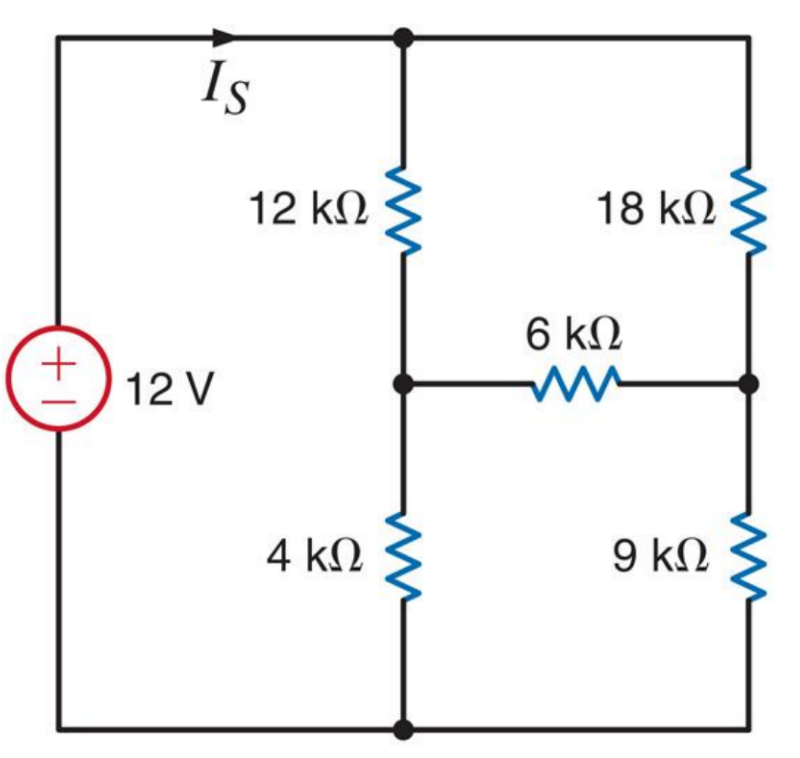
\includegraphics[width=0.7\textwidth]{graphics/ex7/f1.png}
    \caption{Mạch ban đầu}
\end{figure}
\subsection{Biến đổi mạch}
Dễ thấy 3 điện trở \(12k\Omega\), \(18k\Omega\) và \(6k\Omega\) tạo thành mạch \(\Delta\), nên để dễ tính toán hơn thì ta sẽ biến đổi đoạn mạch này về mạch Wye. Cụ thể như hình 7.2.
\begin{figure}[!htbp]
    \centering
    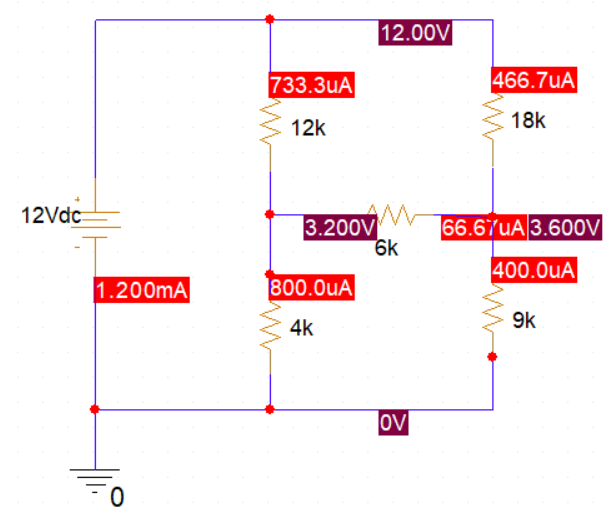
\includegraphics[width=0.7\textwidth]{graphics/ex7/f2.png}
    \caption{Mạch sau khi biến đổi}
\end{figure}
\begin{itemize}
    \item Ta quy ước tên các điện trở trong mạch ban đầu như sau: \(R_a = 6k\Omega,  R_b = 12k\Omega,  R_c = 18k\Omega\).
    \newpage
    \item Tên các điện trở trong mạch sau khi biến đổi được ký hiệu trong hình. Các điện trở mới có giá trị là:
    
    \(R_1 = \frac{R_b \cdot R_c}{R_a + R_b + R_c} = \frac{12k\Omega \cdot 18k\Omega}{6k\Omega + 12k\Omega + 18k\Omega} = 6k\Omega\)

    \(R_2 = \frac{R_a \cdot R_b}{R_a + R_b + R_c} = \frac{6k\Omega \cdot 12k\Omega}{6k\Omega + 12k\Omega + 18k\Omega} = 2 k\Omega\)

    \(R_3 = \frac{R_c \cdot R_a}{R_a + R_b + R_c} = \frac{18k\Omega \cdot 16k\Omega}{6k\Omega + 12k\Omega + 18k\Omega} = 3k\Omega\)
    
\end{itemize}
\subsection{Tính toán}
\begin{itemize}
    \item Sau khi biến đổi, ta dễ dàng tính được điện trở tương đương của mạch:
    
    \(R_{eq} = 6k\Omega + \frac{(3k\Omega + 9k\Omega) \cdot (2k\Omega + 4k\Omega) }{(3k\Omega + 9k\Omega) + (2k\Omega + 4k\Omega)} = 10k\Omega\)
    \item Giá trị dòng điện \(I_S\):
    
    \(I_S = \frac{12V}{R_{eq}} = \frac{12V}{10k\Omega} = 1.2 mA\)

\end{itemize}
\newpage
\subsection{Mô phỏng}
Kết quả mô phỏng:
\begin{figure}[!htbp]
    \centering
    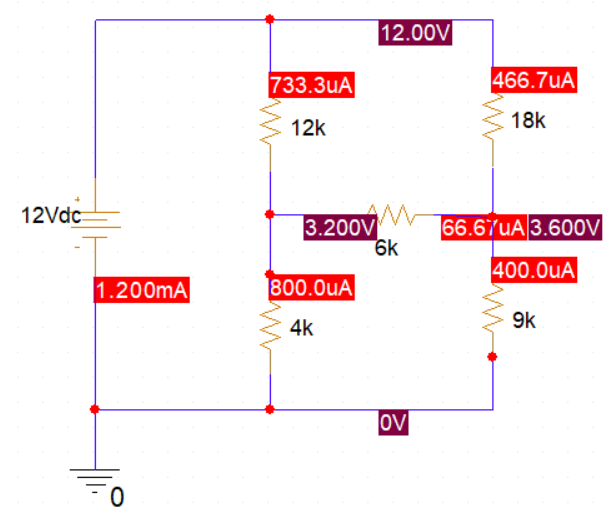
\includegraphics[width=0.7\textwidth]{graphics/ex7/f3.png}
    \caption{Mô phỏng mạch ban đầu}
\end{figure}
\begin{figure}[!htbp]
    \centering
    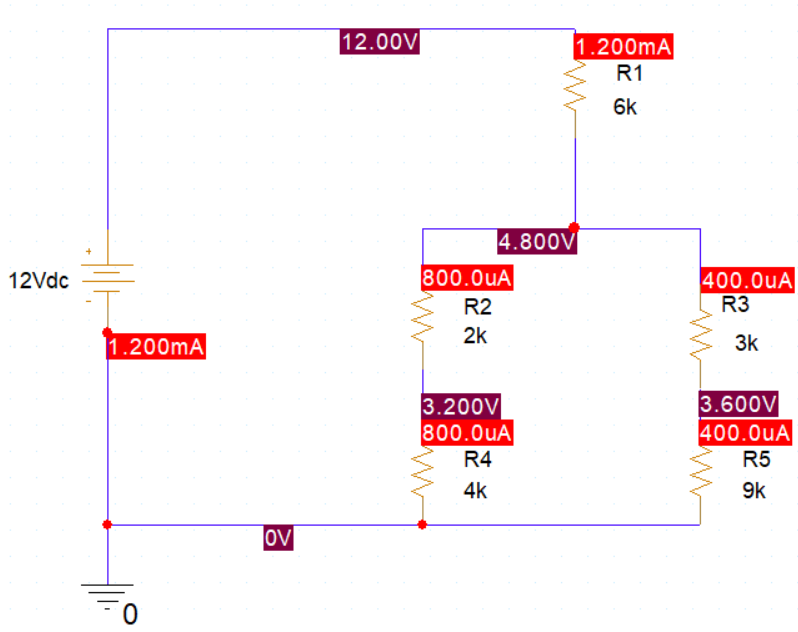
\includegraphics[width=0.7\textwidth]{graphics/ex7/f4.png}
    \caption{Mô phỏng mạch sau khi biến đổi}
\end{figure}